%Anto 
In order to accomplish this project, we have to follow some steps.
First of all we should write the \textbf{Requirement Analysis and Specification Document}. This document helps us to focus on functional and non-functional requirements, domain assumption and goals of the our project.
Thus, we can write the \textbf{Design Document} where we will define the architecture and the component that will be developed.
Then, we start to code the \textbf{Implementation} and in parallel, we write the \textbf{Integration Testing Plan Document}.
Here we explain the strategy we want adopt to test the integration between the system components.
The last document to be released is the \textbf{Project Plan}, that is this document.
After that, we prepare a briefly \textbf{Presentation} of the main part of the previous mentioned document. Finally, when the implementation is almost finished, the \textbf{Integration Test} will be performed.\\
The schedule for each document should observe some deadline definite by our customer. Instead, the implementation phase doesn't have a particular deadline, so we estimate its duration in 13 months, like calculated in section 2. In order to better explain the schedule of the project, we provide a Gantt diagram here below.


\begin{figure}[hp]
  \centering
  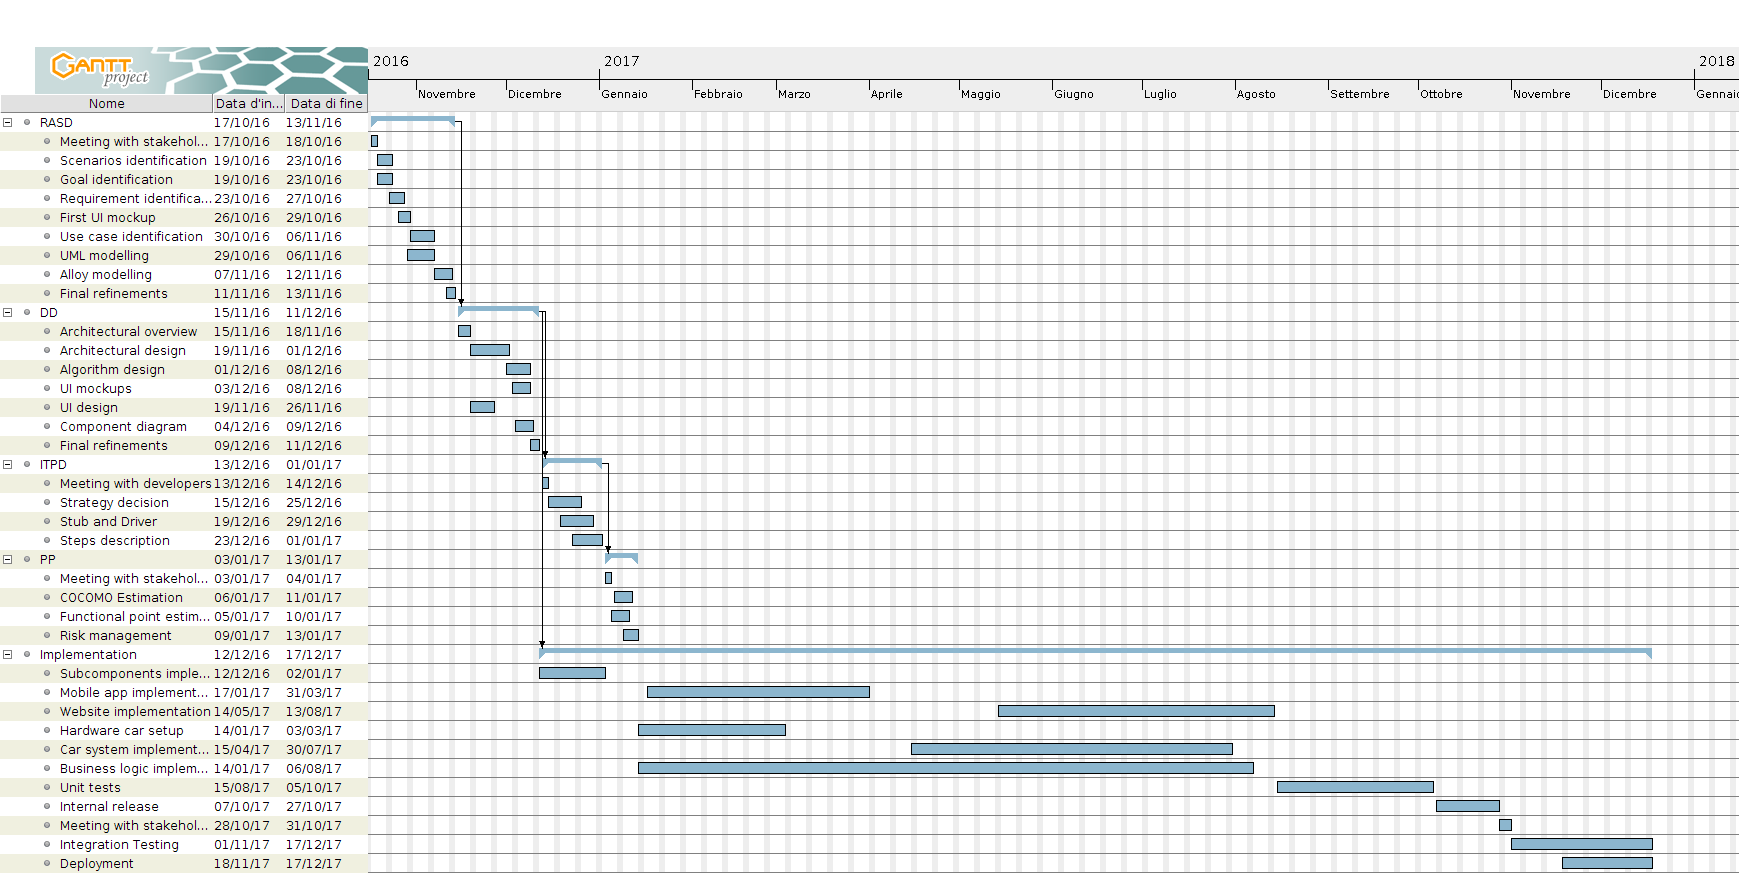
\includegraphics[width=500 pt]{resources/gantt.png}
  \caption{\label{fig:schedule} Gantt diagram for PowerEnJoy project.}
\end{figure}
